\scanpage{60}
\mspage{5}

\figure{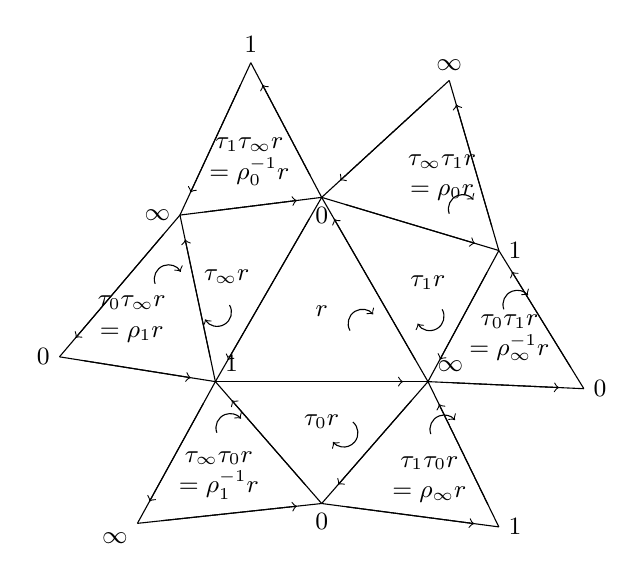
\begin{tikzpicture}[scale=.9,every node/.style={font=\small}]
\coordinate (T) at (0,2.6);\coordinate (L) at (-1.5,0);\coordinate (R) at (1.5,0);
\coordinate (OL) at (-2,2.35);\coordinate (TL) at (-1,4.5);\coordinate (TR) at (1.8,4.25);
\coordinate (OR) at (2.5,1.85);\coordinate (FR) at (3.7,-.1);\coordinate (BR) at (2.5,-2.05);
\coordinate (B) at (0,-1.72);\coordinate (BL) at (-2.6,-2);\coordinate (FL) at (-3.7,.35);
\foreach \p/\q in {T/L,L/R,R/T,T/TL,TL/OL,OL/T,T/OR,OR/TR,TR/T,FL/L,L/OL,OL/FL,FR/OR,OR/R,R/FR,B/L,L/BL,BL/B,B/BR,BR/R,R/B}{\draw (\p)--(\q);\draw[->,shorten >=9pt,shorten <=9pt] (\p)--(\q);}
\node[below] at (T) {$0$};\node[above right] at (L) {$1$};\node[above right] at (R) {$\infty$};
\node[left] at (OL) {$\infty$};\node[above] at (TL) {$1$};\node[above] at (TR) {$\infty$};\node[right] at (OR) {$1$};
\node[right] at (FR) {$0$};\node[right] at (BR) {$1$};\node[below] at (B) {$0$};\node[below left] at (BL) {$\infty$};\node[left] at (FL) {$0$};
\node at (0,1) {$r$};\node at (-1.34,1.48) {$\tau_\infty r$};\node at (1.5,1.4) {$\tau_1r$};\node at (0,-.57) {$\tau_0r$};
\node[align=center] at (-1.02,3.1) {$\tau_1\tau_\infty r$\\$=\rho_0^{-1}r$};
\node[align=center] at (1.7,2.88) {$\tau_\infty\tau_1r$\\$=\rho_0r$};
\node[align=center] at (-2.68,.88) {$\tau_0\tau_\infty r$\\$=\rho_1r$};
\node[align=center] at (2.65,.62) {$\tau_0\tau_1r$\\$=\rho_\infty^{-1}r$};
\node[align=center] at (-1.45,-1.32) {$\tau_\infty\tau_0r$\\$=\rho_1^{-1}r$};
\node[align=center] at (1.52,-1.38) {$\tau_1\tau_0r$\\$=\rho_\infty r$};
\foreach \x/\y/\aa/\bb in {.4/.72/210/40,-1.3/1.08/30/-150,1.7/1.02/30/-150,.44/-.57/50/-140,-2.35/1.38/200/30,2.57/1.02/200/40,1.8/2.37/200/40,-1.48/-.72/200/40,1.54/-.74/200/40}{\draw[->] (\x,\y) arc (\aa:\bb:.2);}
\end{tikzpicture}}

Les propriétés d'orientation de la figure sont les mêmes que celles expliquées p. $2'$, la figure est plus jolie car de nature plus symétrique. \unsure{Du reste}, dans des cas particuliers certains des 10 \deleted{\unsure{triangles}} \inserted{triangles} repères de la figure peuvent coïncider (ex: octaèdre, ou exemple plus dégénéré encore, le cas ``orienté universel''
\figure{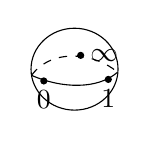
\begin{tikzpicture}[scale=.65]
\draw (0,0) ellipse (.85 and .8);
\draw (-.84,-.12) .. controls (-.25,-.38) and (.45,-.4) .. (.84,-.06);
\draw[dashed] (-.84,-.12) .. controls (-.42,.44) and (.43,.3) .. (.84,-.06);
\fill (-.6,-.23) circle(2pt);\fill (.66,-.2) circle(2pt);\fill (.12,.27) circle(2pt);
\node[below] at (-.6,-.23) {$0$};\node[below] at (.66,-.2) {$1$};\node[right] at (.12,.27) {$\infty$};
\end{tikzpicture}}.

Ici l'équivalence de catégories ad hoc
\diagram{\begin{tikzcd}[column sep=large]
(17)\quad\begin{array}{c}\text{cartes isot. tri-angulaires}\\\text{pondérées}\end{array}\arrow[r,"\approx"]&\begin{array}{c}\Pi_{03}^\tau\text{-ensembles}\\\text{finis spéciaux}\end{array}
\end{tikzcd}}
est en termes des ens finis $R$ à opérateurs involutifs $\tau_i$ ($i\in\{0,1,\infty\}$) \uline{sans points fixes}, sans plus.

Définissant les cartes tri-angulaires pondérées orientées comme dans le cas des cartes ordinaires, par une orientation de la surface top. sous-jacente, on voit que cette notion se définit encore combinatoirement par la donnée d'un sous-ens. $R^+(X)$ de l'ens $R(X)$ des repères pondérés de $X$, satisfaisant (6 bis), i.e. (7), \deleted{bis.}\inserted{(7 bis)} \deleted{\unsure{et}} on a encore posé
\[
R^-(X)=R(X)\setminus R^+(X).
\]
On a alors

\mspage{59}
